\renewcommand{\theequation}{\theenumi}
\begin{enumerate}[label=\arabic*.,ref=\thesubsection.\theenumi]
\numberwithin{equation}{enumi}

\item
Solve
 \begin{align}
 \label{ch2_kkt_problem}
\min_{\mbf{x}} f\brak{\mbf{x}} = \vec{x}^T\myvec{4 & 0 \\0 & 2}\vec{x}
%4x_1^2 + 2x_2^2
 \end{align}
 with constraints
 \begin{align}
 g_1\brak{\mbf{x}} = \myvec{3 & 1}\vec{x}-8 = 0\\
 g_2 \brak{\mbf{x}}= 15 - \myvec{2 & 4}\vec{x} \geq 0
 \end{align}
 
%
\solution Considering the Lagrangian
%
\begin{align}
%L\brak{\mbf{x},\lambda} &= f\brak{\mbf{x}} + \lambda g_1\brak{\mbf{x}} - \mu g_2\brak{\mbf{x}} \\
% &= 4x_1^2 + 2x_2^2 + \lambda \brak{3x_1 + x_2-8} 
% \nonumber \\
% &\,-\mu\brak{15 - 2x_1 - 4x_2},\\
 \nabla L\brak{\mbf{x},\lambda, \mu}  %& = 
%\begin{pmatrix}
%8x_1 + 3 \lambda  +2 \mu  \\
%4x_2 + \lambda + 4 \mu \\
%3x_1 + x_2 -8 \\
% - 2x_1 - 4x_2 + 15
%\end{pmatrix}
= 0
\end{align}
%
resulting in the matrix equation
%
\begin{align}
\Rightarrow 
\begin{pmatrix}
8 &0 & 3 & 2\\
0 &4 & 1 & 4 \\
3 & 1 & 0 &0  \\
2 & 4 & 0 & 0
\end{pmatrix}
\begin{pmatrix}
x_1 \\
x_2 \\
\lambda
\\
\mu
\end{pmatrix}
&=
\begin{pmatrix}
0 \\
0 \\
8 \\
15
\end{pmatrix}
\\
\Rightarrow 
\begin{pmatrix}
x_1 \\
x_2 \\
\lambda
\\
\mu
\end{pmatrix}
&= 
\begin{pmatrix}
1.7 \\
 2.9 \\
-3.12 \\
-2.12
\end{pmatrix}
\end{align}
%
using the following python script.  The (incorrect) graphical solution is available in Fig. \ref{fig.2.12}
%	
\begin{lstlisting}
codes/optimization/2.12.py
\end{lstlisting}

%
Note that $\mu < 0 $, contradicting the necessary condition in \eqref{ch2_kkt_necessary}. 
%
\begin{figure}[!ht]
\centering
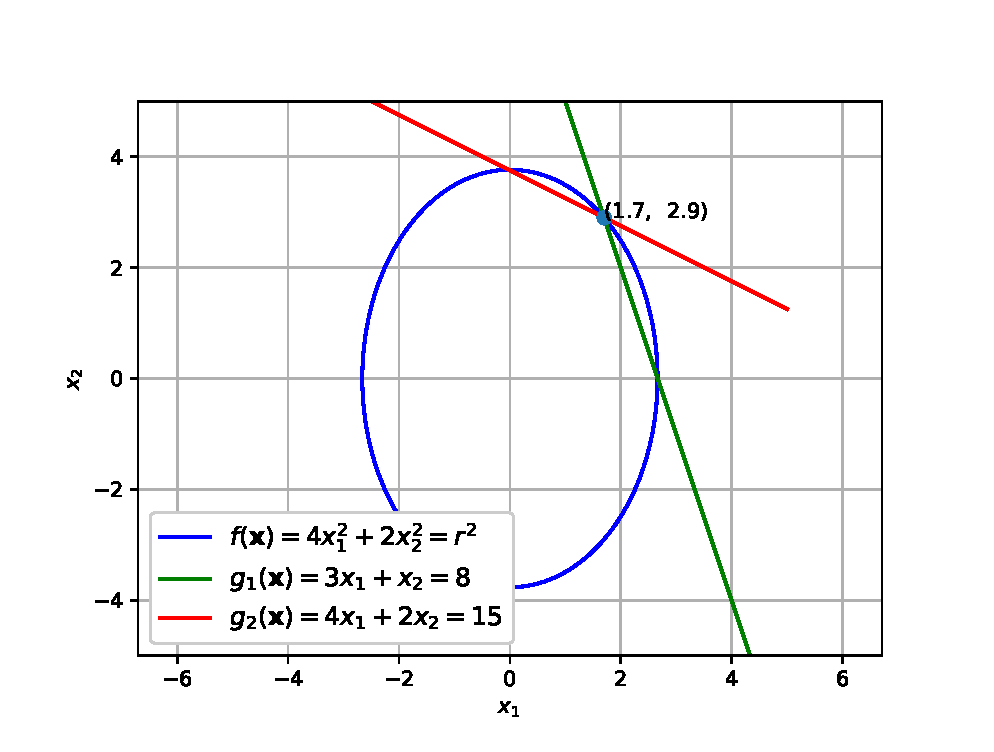
\includegraphics[width=\columnwidth]{./optimization/figs/2.12_1.eps}
\caption{ Incorrect solution is at intersection of all curves $r = 5.33$}
\label{fig.2.12}	
\end{figure}
\item
Obtain the correct solution to the previous problem by considering $\mu = 0$.

\begin{figure}[!ht]
\centering
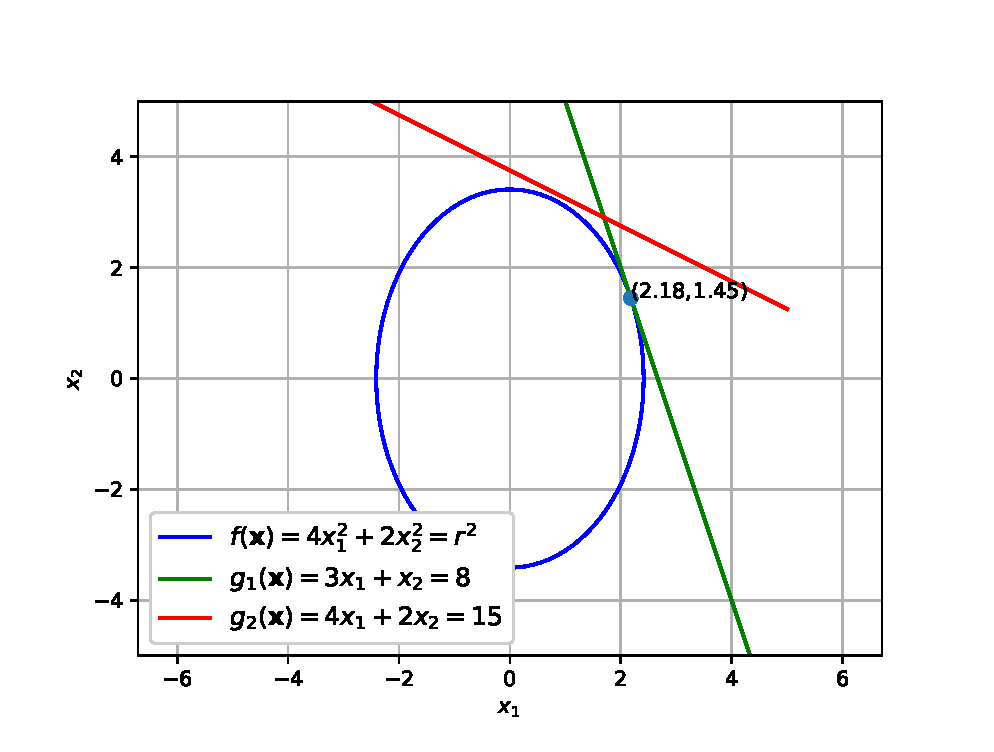
\includegraphics[width=\columnwidth]{./optimization/figs/2.12_2.eps}
\caption{ Optimal solution is where $g_1(x)$ touches the curve $r = 4.82$}
\label{fig.2.13}	
\end{figure}
%
%
\item
Solve
 \begin{align}
% \label{ch2_kkt_problem}
\min_{\mbf{x}} f\brak{\mbf{x}} %= 4x_1^2 + 2x_2^2
 \end{align}
 with constraints
 \begin{align}
 g_1\brak{\mbf{x}} 
%= 3x_1 + x_2-8 
= 0\\
 g_2 \brak{\mbf{x}}
%= 15 - 2x_1 - 4x_2 
\leq 0
 \end{align}
 
%
\item
Based on whatever you have done so far,	list the steps that you would use in general for solving a convex optimization problem  like \eqref{ch2_kkt_problem}  using Lagrange Multipliers. 
These are called Karush-Kuhn-Tucker(KKT) conditions.

\solution For a problem defined by 
\begin{align}
\mbf{x^*} &= \min_{\mbf{x}}f(\mbf{x})
\\
\text{subject to } h_i(\mbf{x}) &= 0, \forall i=1,..,m
\\
\text{subject to } g_i(\mbf{x}) &\le 0, \forall i=1,..,n
\end{align}
%
the optimal solution is obtained through
%
\begin{align}
\mbf{x^*} &= \min_{\mbf{x}}L(\mbf{x}, \mbf{\lambda}, \mbf{\mu}) 
\\
&= \min_{\mbf{x}}f(\mbf{x})  + \underset{i=1}{\overset{m}{\sum}} \lambda_i h_i(\mbf{x}) + \underset{i=1}{\overset{n}{\sum}} \mu_i g_i(\mbf{x}),
\end{align}
%
using the KKT conditions
%
\begin{align}
\Rightarrow \nabla_\mbf{x} f(\mbf{x})  + \underset{i=1}{\overset{m}{\sum}} \nabla_\mbf{x} \lambda_i h_i(\mbf{x}) + \underset{i=1}{\overset{n}{\sum}} \mu_i \nabla_\mbf{x} g_i(\mbf{x}) = 0 
\\
\text{subject to }\mu_i g_i(\mbf{x}) = 0, \forall i = 1,..,n
\\
\text{and }\mu_i \ge 0, \forall i = 1,..,n
\end{align}
%
%
\item
	Maxmimize 
	%
	\begin{align}
	f(\mbf{x}) &= \sqrt{x_1x_2}
	\end{align}
	%
	with the constraints
	%
	\begin{align}
	x_1^2+x_2^2 &\leq 5 \\
	x_1 \geq 0, x_2 &\geq 0
	\end{align}
	%
\end{enumerate}

